\begin{figure}[t]
 	\centering
 	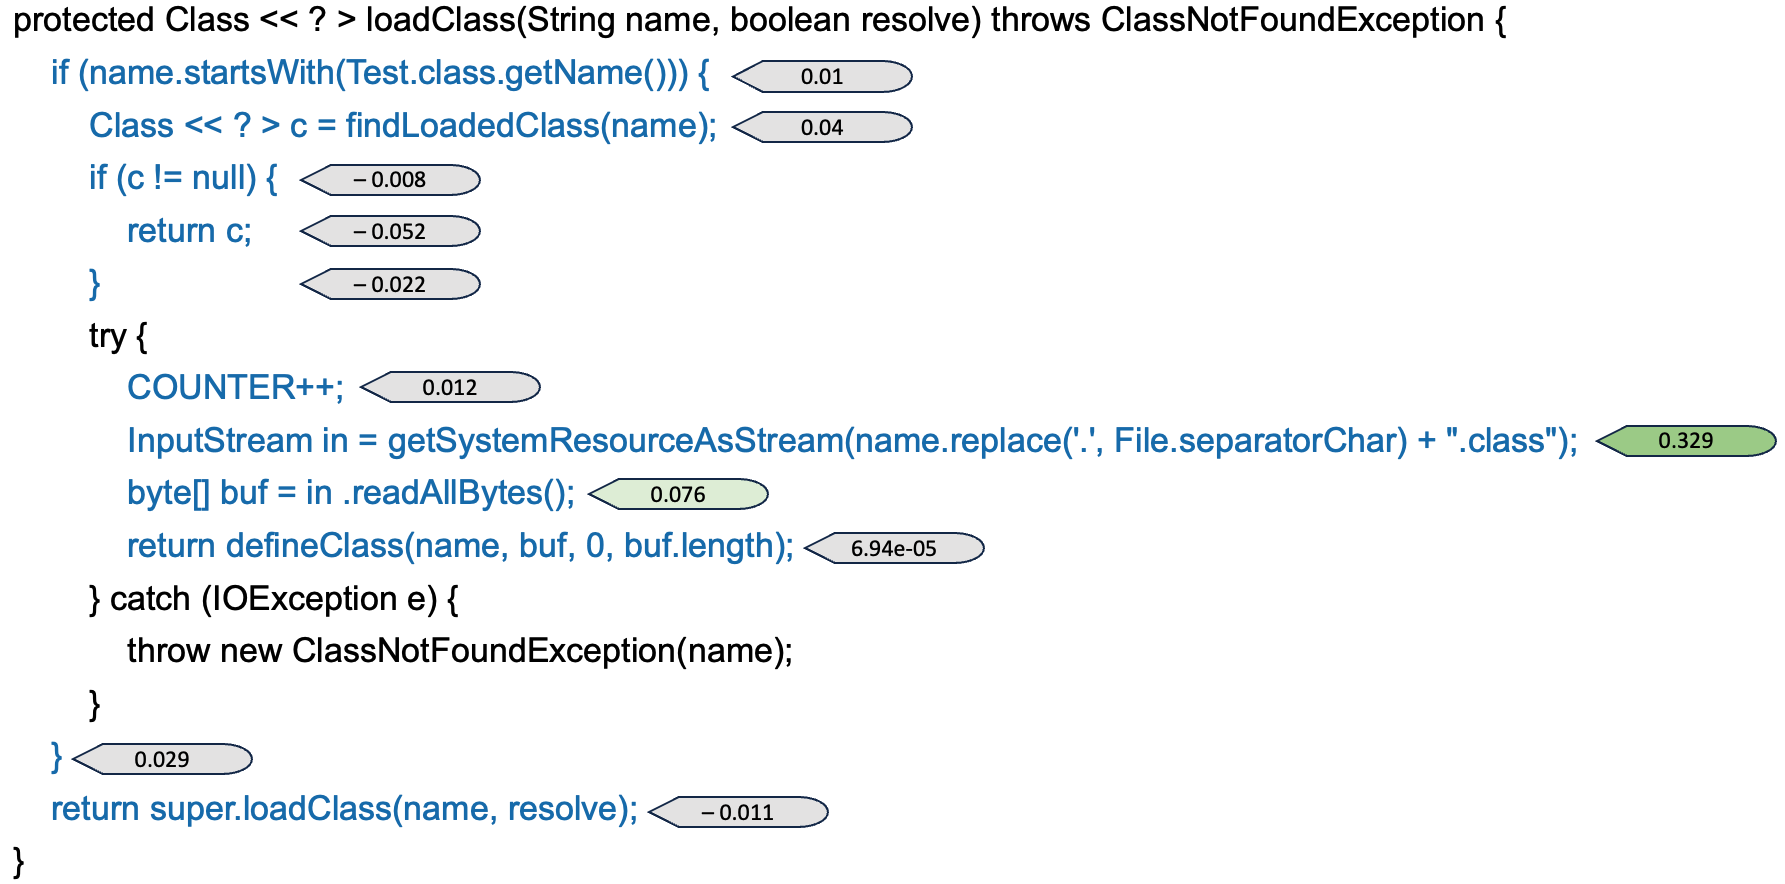
\includegraphics[width=3.4in]{rq1-case-study.png}
        \vspace{-20pt}
 	\caption{{\xblock} Case Study}
 	\label{fig:rq1-case}	
\end{figure}

To illustrate how {\xblock} makes the prediction, in Figure~\ref{fig:rq1-case}, we shows a code snippet that catches an IOException thrown by the \code{readAllBytes} function call on a \code{InputStream} object. The number after each statement is the statement attribution score, which is calculated by averaging the attribution scores of all the sub-tokens in the statement. A positive score means that the statement contributes positively to the model's predicted class, while a negative score means the statement contributes negatively to the predicted class.  As we can see, the two statements that receive the highest scores are the statement that defines the \code{InputStream} variable and the statement that invokes the \code{readAllBytes} function call on the \code{InputStream} object. 